\subsubsubsection{Recurrent Neural Network}
\\\\
\indent Развивая тему особенностей архитектур сетей, задаемся вопросом: \textbf{Q}: MLP работает с матрицей вида объект---признак, однако как поступать в случае работы с временным рядом, ведь исходный его вид --- просто вектор? \textbf{A}: Как уже отмечалось в блоке Singular Spectrum Analysis (\myref{link::ssa}), переводим имеющийся ряд (вектор) в матричное пространство посредством применения алгоритма подобного ханкелизации. Таким образом, вместо временного ряда $y \in \R^{N}$, получаем матрицу $y \in \R^{L \times K}$, где $K  = N - L$. Для большей наглядности рассматриваем пример.
\begin{equation}
	\begin{split}
		y = \left[\begin{matrix}
			1\\2\\3\\4\\5\\6
		\end{matrix}\right], L = 4, K = 6 - 4 = 2 \Rightarrow
		X = \left[\begin{matrix}
			1 & 2\\
			2 & 3\\
			3 & 4\\
			4 & 5\\
		\end{matrix}\right]
		y = \left[\begin{matrix}
			3\\
			4\\
			5\\
			6\\
		\end{matrix}\right]
	\end{split}	
\end{equation}
Получаем то, что было нужно. Матрица объект-признак ($X$) и вектор выходов ($y$), который должен быть в итоге. Однако снова появляется вопрос \textbf{Q}: Так как работа ведется с временным рядом, целесообразно ли иметь фиксированный набор признаков, который подается на вход сети. В текущих условиях входной размерностью сети является величина $K$ (количество временных лагов). Но, что будет, если два лага найдутся не всегда? \textbf{A}: Решением этой проблемы является способ построения нейронных сетей, предложенный в \cite{hochreiter1997long, rumelhart1986learning}, представляющий из себя последовательный сбор информации о последовательности. Данный поход получил название Recurrent Neural Network (рекуррентная нейронная сеть).

Идея в том, что на вход аналогично всем предыдущему подается наблюдение, однако, рассуждая абстрактно, имеет в виду не просто \textit{одно} наблюдение, а последовательность из них. Для лучшего понимания происходящего рассматриваем примере выше. Чтобы перевести имеющиеся $X$ и $y$ в требуемые для RNN размерности, выполняем операцию:
\begin{equation}
	\begin{split}
		X = \left[\begin{matrix}
			1 & 2\\
			2 & 3\\
			3 & 4\\
			4 & 5\\
		\end{matrix}\right]
		y = \left[\begin{matrix}
			3\\
			4\\
			5\\
			6\\
		\end{matrix}\right]
		\Rightarrow
		X = \left[\begin{matrix}
			[1], & [2]\\
			[2], & [3]\\
			[3], & [4]\\
			[4], & [5]\\
		\end{matrix}\right]
		y = \left[\begin{matrix}
			[3]\\
			[4]\\
			[5]\\
			[6]\\
		\end{matrix}\right]
	\end{split}	
\end{equation}
То есть теперь $X \in \R^{L \times K \times 1}$, а значит, приводя все в соответствие необходимой терминологии, $L$ --- размер батча, $K$ --- длина последовательности, $1$ --- количество имеющихся признаков у одного наблюдения, в нашем случае --- цена акции открытия, однако возможно наличие и других составляющих. А теперь самое интересное: подобная архитектура требует лишь фиксированного количества признаков у одного наблюдения, в то время как длина последовательности --- количество лагов, в нашем случае --- остается динамической. Следовательно не нужно менять архитектуру сети в зависимости от количества используемых лагов --- в зависимости от длины последовательности. Данные подготовлены, теперь приступаем к систематическому изложению особенности работы алгоритма RNN.

Существует три на данный момент существующих основных блока рекуррентных сетей: Simple Recurrent Unit \cite{rumelhart1986learning}, Long Short Term Memory (LSTM) \cite{hochreiter1997long}, Gated Recurrent Unit (GRU) \cite{cho2014learning}. Коротко говоря о каждом из них, привожу иллюстративный способ работы блоков, а также формальные вычисления.

Для начала --- Simple Recurrent Unit:
\begin{figure}[H]
	\centering
	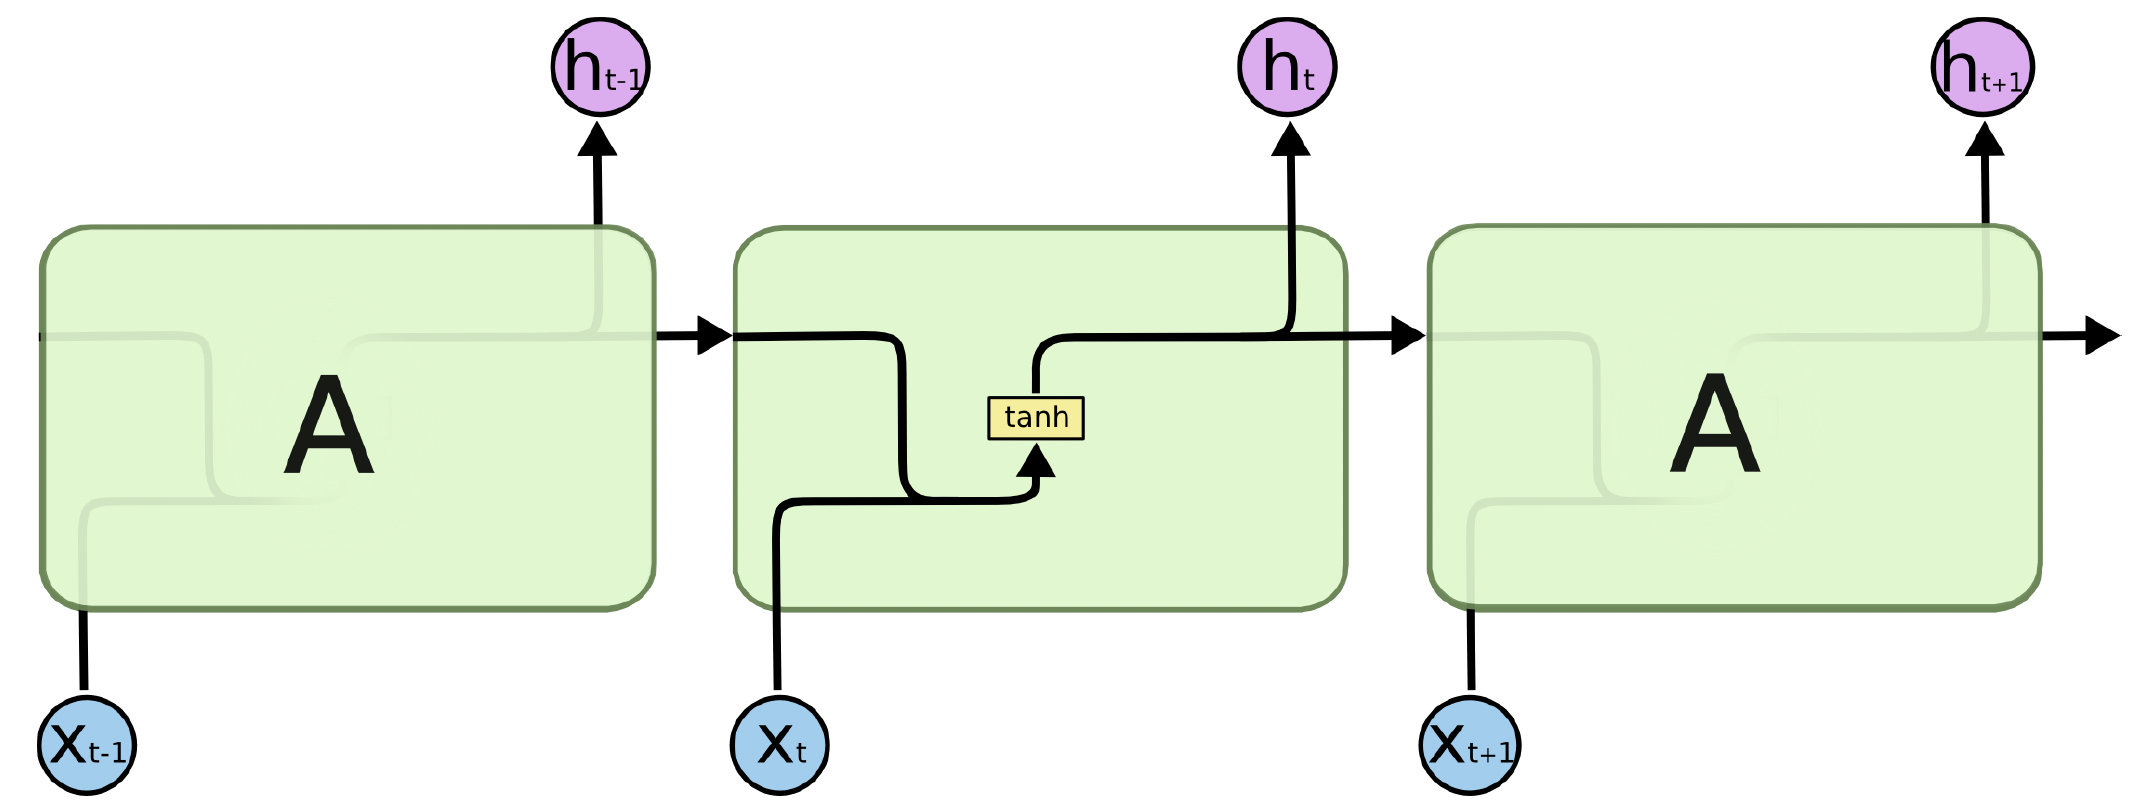
\includegraphics[width=17cm]{nn/rnn/units/rnn_unit.png}
	\caption{Визуализация блока Simple Recurrent Unit}
	\label{fig::rnn_unit}
\end{figure}
\noindent В формальном виде, вычисления проходят следующим образом:
\begin{equation}
	\begin{split}
		h_t & = \sigma\left(W_{hh}h_{t - 1} + W_{hx} x_t + b_h\right)\\
		y_ t & = g\left(W_{yh}h_t + b_y\right)
	\end{split}
\end{equation}
Но тут сразу встает вопрос о затухании градиента при обратном проходе, то есть при применении так называемого алгоритма BackPropagation Through Time (BPTT), являющегося аналогичным классическому BackPropagation \cite{linnainmaa1970representation}. Формально данный вывод получаем посредством дифференцирования выбранной функции потерь:
\begin{equation}
	\begin{split}
		\frac{\partial L}{\partial w} = \sum_{t = 1}^T  \frac{\partial h_k}{\partial w} \left\{ \prod_{i = k + 1}^{t} \frac{\partial h_i}{\partial h_{i - 1}}\right\} \frac{\partial y_t}{\partial h_t} \frac{\partial L}{\partial y_t}
	\end{split}
\end{equation}
При этом если $\lVert \frac{\partial h_i}{\partial h_{i - 1}} \rVert_2 > 1 \Rightarrow$ взрыв, иначе $\lVert \frac{\partial h_i}{\partial h_{i - 1}} \rVert_2 < 1 \Rightarrow$ затухание в силу наличия произведения матриц Якоби. При этом --- желаемый результат --- $\lVert \frac{\partial h_i}{\partial h_{i - 1}} \rVert_2 = 1$. Решением появившейся проблемы стало изобретение в 1991 блока Long Short Term Memory, описанного в \cite{hochreiter1991untersuchungen, hochreiter1997long}. В формальном виде процесса вычислений получаем:
\begin{equation}
	\begin{split}
		f_t & = \sigma \left(W_{hh}^f h_{t - 1} + W_{hx}^f x_t + b_h^f\right)\\
		i_t & = \sigma \left(W_{hh}^i h_{t - 1} + W_{hx}^i x_t + b_h^i\right)\\
		o_t & = \sigma \left(W_{hh}^o h_{t - 1} + W_{hx}^o x_t + b_h^o\right)\\
		\tilde{c}_t & = \tanh\left(W_{hh}^c h_{t - 1} + W_{hx}^c x_t + b_c\right)\\
		c_t & = f_t c_{t - 1} + i_{t} \tilde{c}_t\\
		h_t & = o_t \tanh\left(c_t\right)
	\end{split}
\end{equation}
\noindent Графически же иллюстрация вычислительного процесс имеет более сложный вид, чем выше упомянутый Simple Recurrent Unit, однако сложность архитектуры окупается способностью данного блока избегать проблемы затухания градиента, а также --- способностью вычленять долгосрочные зависимости в имеющихся данных (в терминах сигналов --- выделение тренда).
\begin{figure}[H]
	\centering
	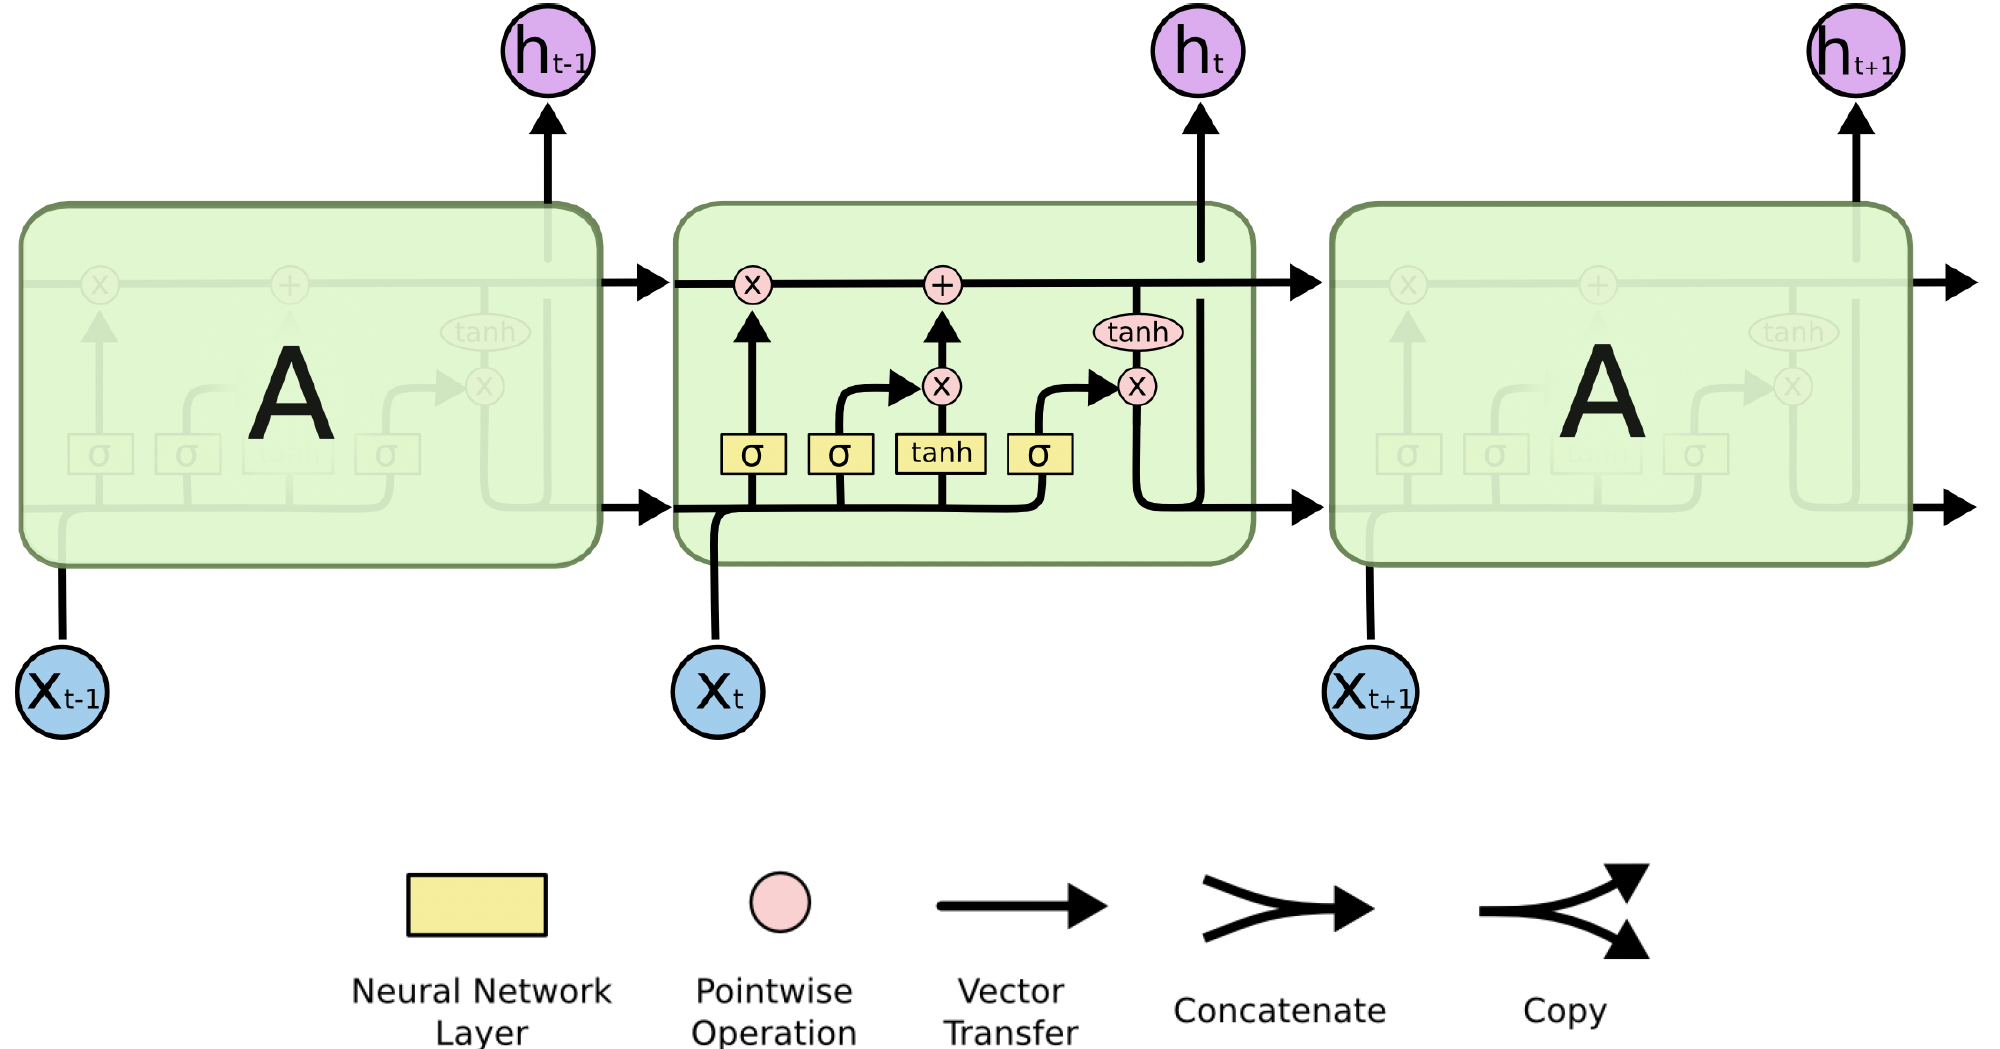
\includegraphics[width=17cm]{nn/rnn/units/lstm_unit.png}
	\caption{Визуализация блока Long Short Term Memory}
	\label{fig::lstm_unit}
\end{figure}
Как видим, проблема с затуханием градиента решена, однако блок получился достаточно тяжелым с точки зрения вычислений и, более того, проблема <<взрыва>> градиента никуда не делать. Вторая трудность решается посредством приема, называемого gradient clipping \cite{mikolov2012statistical}, а первая, в свою очередь, посредством далее изобретенного в 2014 блока Gated Recurrent Unit \cite{cho2014learning}, который по качеству работы сравним с LSTM, но при этом является более <<легким>> в плане количества обучаемых параметров. Формулы данного процесса:
\begin{equation}
	\begin{split}
		z_t & = \sigma\left(W_{hh}^i h_{t - 1} + W_{hx}^i x_t + b_h^z\right)\\
		r_t & = \sigma\left(W_{hh}^r h_{t - 1} + W_{hx}^r x_t + b_h^r\right)\\
		\tilde{h}_t & = \tanh \left(W_{hh}^r h_{t - 1} + W_{hx}^r x_t\right)\\
		h_t & = (1 - z_t) h_{t - 1} + z_t \tilde{h}_t
	\end{split}
\end{equation}
\noindent Визуально реализация блока GRU выглядит намного легче в плане количества параметров, чем LSTM, что позволяет предполагать увеличение скорости обучения сети, но при это сохранение качества получаемых результатов.
\begin{figure}[H]
	\centering
	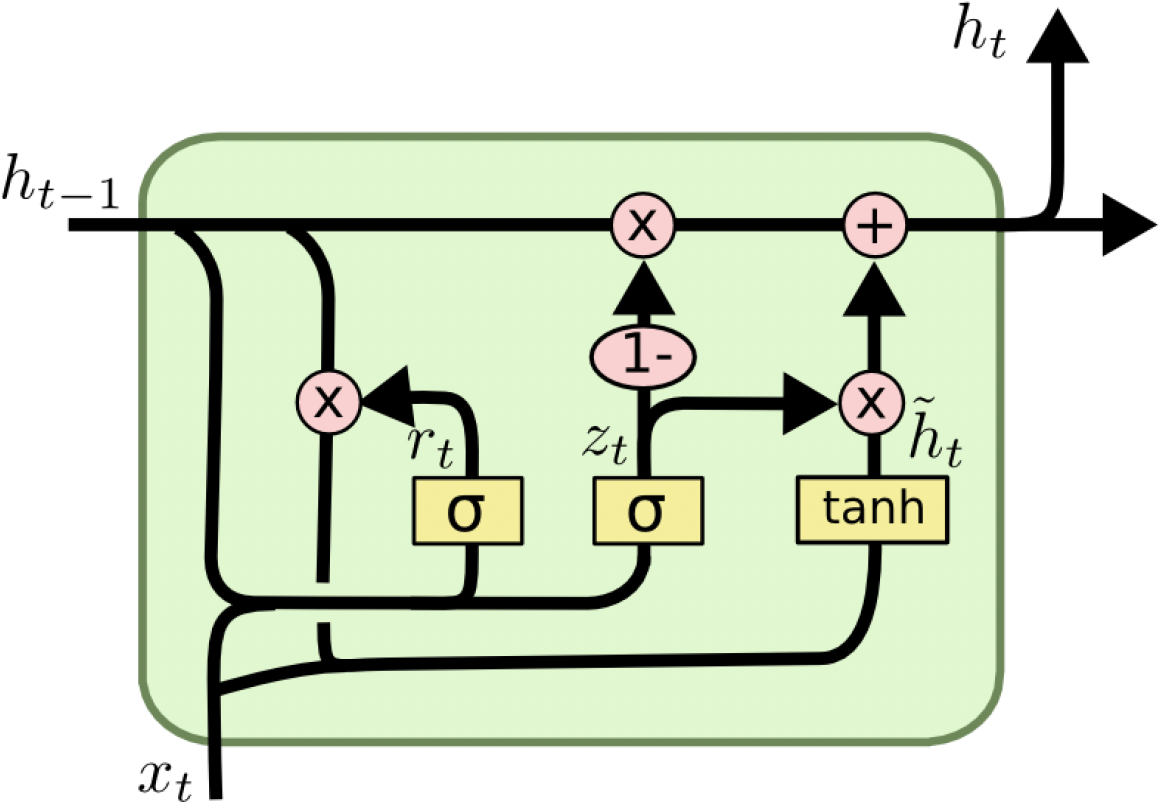
\includegraphics[width= 8cm]{nn/rnn/units/gru_unit.png}
	\caption{Визуализация блока Gated Recurrent Unit}
	\label{fig::gru_unit}
\end{figure}
Несмотря на все достоинства GRU перед LSTM невозможно однозначно сказать, какой из указанных блоков лучше. Таким образом, остается лишь один способ проверки --- эмпирически на имеющихся данных. В настоящей работе в качестве примера приводится эмпирический анализ каждого из выше указанных блоков на имеющихся данных о ценах открытия компании Ford.

Ниже приводим полученные результаты для блока Simple Recurrent Unit.
\begin{figure}[H]
	\centering
	\includegraphics[width= 17cm]{nn/rnn/block_results/rnn/ford_train_val_prices.png}
	\caption{График MSE для блока Simple Recurrent Unit (цены USD)}
	\label{fig::rnn_ford_train_val_prices}
\end{figure}
\noindent Далее смотрим на динамику лучшей валидационной метрики за все время обучения:
\begin{figure}[H]
	\centering
	\includegraphics[width= 17cm]{nn/rnn/block_results/rnn/ford_best_metric_prices.png}
	\caption{График изменения лучшей валидационной метрики: WAPE}
	\label{fig::rnn_ford_best_metric_prices}
\end{figure}
\noindent Далее --- предсказания:
\begin{figure}[H]
	\centering
	\includegraphics[width= 17cm]{nn/rnn/block_results/rnn/ford_test_prices.png}
	\caption{График реальных и предсказанных цен акций Ford (USD)}
	\label{fig::rnn_ford_test_prices}
\end{figure}
\noindent Аналогичный анализ для доходностей.
\begin{figure}[H]
	\centering
	\includegraphics[width= 17cm]{nn/rnn/block_results/rnn/ford_train_val_returns.png}
	\caption{График MSE для блока Simple Recurrent Unit (доходности \%)}
	\label{fig::rnn_ford_train_val_returns}
\end{figure}
\noindent Смотрим на динамику лучшей валидационной метрики за все время обучения:
\begin{figure}[H]
	\centering
	\includegraphics[width= 17cm]{nn/rnn/block_results/rnn/ford_best_metric_returns.png}
	\caption{График изменения лучшей валидационной метрики: WAPE}
	\label{fig::rnn_ford_best_metric_returns}
\end{figure}
\noindent Далее --- предсказания:
\begin{figure}[H]
	\centering
	\includegraphics[width= 17cm]{nn/rnn/block_results/rnn/ford_test_returns.png}
	\caption{График реальных и предсказанных доходностей Ford (\%)}
	\label{fig::rnn_ford_test_returns}
\end{figure}
\noindent Таким образом, для цен --- $0.5$ USD, что заметно меньше, чем было для MLP ($1.29$ USD), а для доходностей $2.91\%$, что больше, чем для MLP ($1.99\%$). Результат для доходностей все равно не применим к реальной жизни, так как показывает отклонение выше, чем среднюю. Далее рассматриваем работу блока GRU. Аналогично: вначале цены, затем доходности.
\begin{figure}[H]
	\centering
	\includegraphics[width= 17cm]{nn/rnn/block_results/gru/ford_train_val_prices.png}
	\caption{График MSE для блока Gated Recurrent Unit (цены USD)}
	\label{fig::gru_ford_train_val_prices}
\end{figure}
\noindent Валидационная метрика за все время обучения:
\begin{figure}[H]
	\centering
	\includegraphics[width= 17cm]{nn/rnn/block_results/gru/ford_best_metric_prices.png}
	\caption{График изменения лучшей валидационной метрики: WAPE}
	\label{fig::gru_ford_best_metric_prices}
\end{figure}
\noindent Далее --- предсказания:
\begin{figure}[H]
	\centering
	\includegraphics[width= 17cm]{nn/rnn/block_results/gru/ford_test_prices.png}
	\caption{График реальных и предсказанных цен акций Ford (USD)}
	\label{fig::gru_ford_test_prices}
\end{figure}
\noindent Аналогичный анализ для доходностей.
\begin{figure}[H]
	\centering
	\includegraphics[width= 17cm]{nn/rnn/block_results/gru/ford_train_val_returns.png}
	\caption{График MSE для блока Gated Recurrent Unit (доходности \%)}
	\label{fig::gru_ford_train_val_returns}
\end{figure}
\noindent Динамика лучшей валидационной метрики:
\begin{figure}[H]
	\centering
	\includegraphics[width= 17cm]{nn/rnn/block_results/gru/ford_best_metric_returns.png}
	\caption{График изменения лучшей валидационной метрики: WAPE}
	\label{fig::gru_ford_best_metric_returns}
\end{figure}
\noindent Далее --- прогнозы:
\begin{figure}[H]
	\centering
	\includegraphics[width= 17cm]{nn/rnn/block_results/gru/ford_test_returns.png}
	\caption{График реальных и предсказанных доходностей Ford (\%)}
	\label{fig::gru_ford_test_returns}
\end{figure}
Соответственно, ошибка на ценах получилась больше на $0.05$ USD, чем у Simple Recurrent Unit ($0.5$ USD) однако ошибка на доходностях уменьшилась до $2.89\%$, что меньше на $0.1\%$ пунктов. Далее анализируем блок LSTM.
 \begin{figure}[H]
 	\centering
 	\includegraphics[width= 17cm]{nn/rnn/block_results/lstm/ford_train_val_prices.png}
 	\caption{График MSE для блока LSTM (цены USD)}
 	\label{fig::lstm_ford_train_val_prices}
 \end{figure}
 \noindent Валидационная метрика за все время обучения:
 \begin{figure}[H]
 	\centering
 	\includegraphics[width= 17cm]{nn/rnn/block_results/lstm/ford_best_metric_prices.png}
 	\caption{График изменения лучшей валидационной метрики: WAPE}
 	\label{fig::lstm_ford_best_metric_prices}
 \end{figure}
 \noindent Прогнозы:
 \begin{figure}[H]
 	\centering
 	\includegraphics[width= 17cm]{nn/rnn/block_results/lstm/ford_test_prices.png}
 	\caption{График реальных и предсказанных цен акций Ford (USD)}
 	\label{fig::lstm_ford_test_prices}
 \end{figure}
 \noindent Анализ доходностей.
 \begin{figure}[H]
 	\centering
 	\includegraphics[width= 17cm]{nn/rnn/block_results/lstm/ford_train_val_returns.png}
 	\caption{График MSE для блока LSTM (доходности \%)}
 	\label{fig::lstm_ford_train_val_returns}
 \end{figure}
 \noindent Динамика лучшей валидационной метрики:
 \begin{figure}[H]
 	\centering
 	\includegraphics[width= 17cm]{nn/rnn/block_results/lstm/ford_best_metric_returns.png}
 	\caption{График изменения лучшей валидационной метрики: WAPE}
 	\label{fig::lstm_ford_best_metric_returns}
 \end{figure}
 \noindent Предсказания:
 \begin{figure}[H]
 	\centering
 	\includegraphics[width= 17cm]{nn/rnn/block_results/lstm/ford_test_returns.png}
 	\caption{График реальных и предсказанных доходностей Ford (\%)}
 	\label{fig::lstm_ford_test_returns}
 \end{figure}
 Видим увеличение ошибки для цен на $0.07$ USD по сравнению с Simple Recurrent Unit, а также увеличение ошибки для доходностей до $2.90\%$ по сравнению с Gated Recurrent Unit ($2.89\%$).
 
 Выводом ко всему вышеописанному является то, что применение Simple Recurrent Unit для работы с ценами --- вестма неплохая идея, так как RMSE метрика уменьшилась примерно в 2 раза, однако применение какого-либо блока из класса Recurrent Network не является целесообразным для прогнозирования доходностей, тут лучше всего справляется классическая MLP модель ($1.99\%$). Однако, подводя итог, ни одна из моделей не годится для работ с доходностями в полевых условиях, так как отклонение прогнозируемого значения от реального превышает само прогнозируемое значение, таким образом, нельзя точно быть уверенными, как именно себя поведет доходность.
 
 В заключении данного блока, рассмотренная модель включается в финальную сравнительную таблицу, однако точно сказать, какой именно блок необходимо использовать --- не получится, так как в среднем результаты почти одинаковые. Соответственно, основываясь на данных, проверяем валидность того или иного блока и далее --- используем его при обучении модели.